\documentclass[14pt, a4paper]{article}
\usepackage[T2A]{fontenc}
\usepackage[utf8]{inputenc}
\usepackage[russian]{babel}
\usepackage[left=3cm, right=1.5cm, top=2cm, bottom=2cm]{geometry}
\usepackage{indentfirst}
\usepackage{microtype}
\usepackage{array}
\usepackage{xcolor}
% \usepackage{times}
\usepackage{tempora}
\usepackage{ulem}
\usepackage{setspace}
\usepackage{amsmath}
\usepackage{booktabs}
\usepackage{graphicx}
\usepackage{float}
\usepackage{listings}
\graphicspath{{reports/figures/}{figures/}}
\lstset{basicstyle=\ttfamily\small, breaklines=true, columns=fullflexible, frame=single, keepspaces=true}
\pagestyle{empty}

\makeatletter
\renewcommand\section{\@startsection {section}{1}{\parindent}%
  {-3.5ex \@plus -1ex \@minus -.2ex}%
  {0.5ex}%
  {\normalfont\Large\bfseries}}
\renewcommand\tableofcontents{%
  \begin{center}\Large\bfseries\contentsname\end{center}%
  \@starttoc{toc}%
}
\renewcommand*\l@section{\@dottedtocline{1}{0em}{1.5em}}
\makeatother

\begin{document}
\onehalfspacing

\begin{center}
    \textbf{ФЕДЕРАЛЬНОЕ ГОСУДАРСТВЕННОЕ АВТОНОМНОЕ ОБРАЗОВАТЕЛЬНОЕ} \\
    \textbf{УЧРЕЖДЕНИЕ ВЫСШЕГО ОБРАЗОВАНИЯ} \\
    \textbf{«МОСКОВСКИЙ АВИАЦИОННЫЙ ИНСТИТУТ} \\
    \textbf{(НАЦИОНАЛЬНЫЙ ИССЛЕДОВАТЕЛЬСКИЙ УНИВЕРСИТЕТ)»}
\end{center}

\begin{center}
    \bfseries Институт №8 «Компьютерные науки и \\
    \bfseries прикладная математика» \\
    \bfseries Кафедра 806 «Вычислительная математика \\
    \bfseries и программирование»
\end{center}

\vspace{3cm}

\begin{center}
    \Large\bfseries Отчет \\
    \vspace{0.5cm}
    \mdseries по лабораторной работе №2.1
\end{center}

\vfill

\noindent
\hfill
\begin{tabular}{ll}
Группа:       & М8О-307Б-21 \\
Студент:      & М. С. Ивченко \\
Преподаватель:& доц. В. В. Киндинова \\
Оценка:       & \underline{\makebox[3cm][c]{}} \\ [0.2cm]
Дата:         & \underline{\makebox[3cm][c]{}}
\end{tabular}

\vfill

\begin{center}
    Москва \\
    2026
\end{center}

\newpage

\setcounter{tocdepth}{2}
\tableofcontents
\newpage

\section*{Тема}
\addcontentsline{toc}{section}{Тема}
Цель данной лабораторной работы -- изучить численные способы нахождения корней нелинейных уравнений. В работе рассматриваются метод простой итерации и метод Ньютона, сравнивается их поведение и оценивается влияние начального приближения на скорость сходимости.

\section*{Задание}
\addcontentsline{toc}{section}{Задание}
Реализовать методы простой итерации и Ньютона решения нелинейных уравнений в виде программ, задавая в качестве входных данных точность вычислений. С использованием разработанного программного обеспечения найти положительный корень нелинейного уравнения (начальное приближение определить графически). Проанализировать зависимость погрешности вычислений от количества итераций.

\section*{Теория}
\addcontentsline{toc}{section}{Теория}
Задача состоит в нахождении такого $x^*$, что $f(x^*)=0$. Перед применением численного метода обычно строят график функции или анализируют смену знака на отрезке, чтобы выбрать область, где находится нужный корень. Если $f(a)f(b)<0$ и функция непрерывна, на отрезке $[a,b]$ есть хотя бы один корень.

Метод Ньютона использует линеаризацию функции в текущей точке. Касательная к графику $f(x)$ в точке $x_k$ пересекает ось абсцисс в следующем приближении:
\[
    x_{k+1}=x_k-\frac{f(x_k)}{f'(x_k)}.
\]
Если начальное приближение достаточно близко к простому корню и $f'(x^*)\ne0$, метод имеет квадратичную сходимость: число верных знаков примерно удваивается на каждой итерации. Однако при плохом начальном приближении или при малой производной шаг может увести итерации от корня.

Метод простой итерации требует записи уравнения в виде
\[
    x=\varphi(x), \qquad x_{k+1}=\varphi(x_k).
\]
Достаточное условие сходимости на отрезке -- условие сжатия:
\[
    |\varphi'(x)|\le q<1.
\]
Тогда итерации остаются в окрестности корня, а погрешность можно оценивать через разность соседних приближений:
\[
    |x^*-x_k|\le \frac{q}{1-q}|x_k-x_{k-1}|.
\]

В реализации для простой итерации использовалась релаксационная форма $\varphi(x)=x-\lambda f(x)$ с автоматическим выбором $\lambda$.
Параметр $\lambda$ подбирается так, чтобы уменьшить максимум $|\varphi'(x)|=|1-\lambda f'(x)|$ на выбранном отрезке. Для обоих методов остановка выполняется при малом изменении приближения или малой невязке $|f(x_k)|$.

\begin{lstlisting}[language=Python]
x_next = x_curr - func(x_curr) / deriv(x_curr)
if abs(x_next - x_curr) < precision_epsilon:
    return x_next
\end{lstlisting}

\section*{Ход лабораторной работы}
\addcontentsline{toc}{section}{Ход лабораторной работы}
Рассматривалось уравнение
\[
    e^x-x^3+3x^2-2x-3=0.
\]
По графику положительный корень находится на отрезке $[0.5,1.5]$, начальное приближение выбрано $x_0=1$.

\begin{figure}[H]
    \centering
    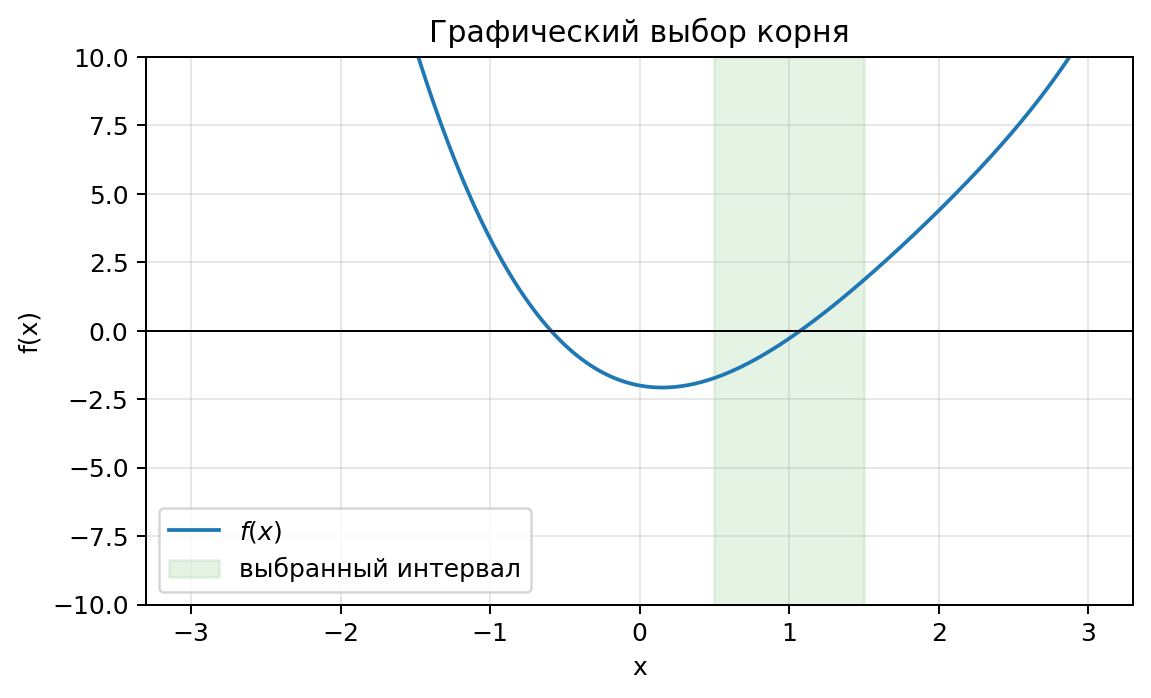
\includegraphics[width=0.86\textwidth]{lab2_1_function.png}
    \caption{Графический выбор начального приближения для положительного корня.}
\end{figure}

Метод Ньютона дал $x=1.0738314383$, невязка $|f(x)|=1.74\cdot10^{-12}$. Метод простой итерации с автоматическими параметрами $\lambda=0.301640$ и $q=0.427269$ дал $x=1.0738432291$. Попытка использовать явную функцию $\varphi(x)=(e^x-x^3+3x^2-3)/2$ не сошлась, так как на выбранном отрезке $q\approx3.37>1$.

\begin{figure}[H]
    \centering
    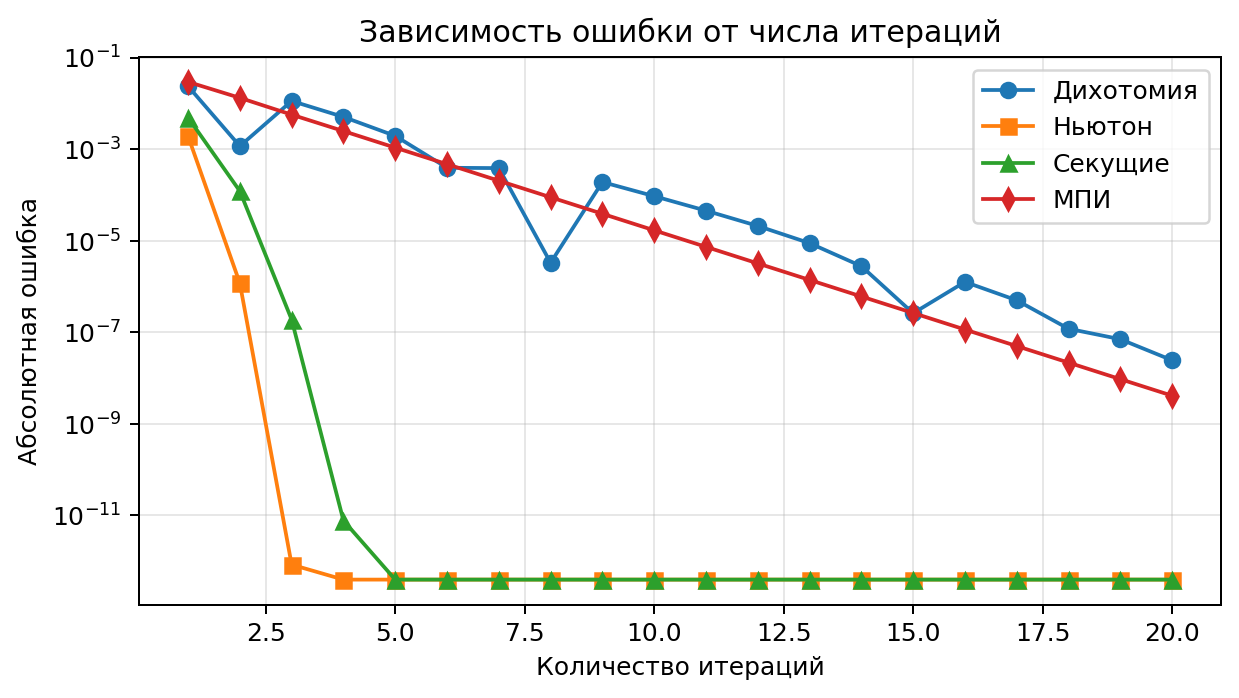
\includegraphics[width=0.86\textwidth]{lab2_1_errors.png}
    \caption{Сравнение убывания ошибки для нескольких методов решения одного уравнения.}
\end{figure}

\section*{Выводы}
\addcontentsline{toc}{section}{Выводы}
Метод Ньютона оказался самым быстрым для выбранного начального приближения. Метод простой итерации чувствителен к выбору функции $\varphi$: релаксационная форма сходится, а естественная перестановка уравнения нарушает условие сжатия.

\end{document}
